\chapter*{Capítulo I}
\addtocontents{toc}{\protect\contentsline{chapter}{Capítulo I}{\thepage}{}}
\setcounter{chapter}{1} % Set the chapter counter to ensure proper numbering
\fancyhf{}
\rhead{Capítulo I}
\lhead{Informe de práctica Inicial en Air Logistics Corp.}
\fancyfoot[R]{\thepage} 
\section{Introducción}
En el presente informe se resumirá las actividades y el aprendizaje durante la práctica inicial del estudiante Eliecer Chavez en la empresa Air Logistics Corp. Se introducirá a la empresa, su rubro, sus necesidades y cómo se aportó a la solución y/o mejoramiento de estos.
\section{Antecedentes Institucionales}

Air Logistics Corp. es una empresa que pertenece a la industria de la aviación. Es una empresa hermana de la empresa A\&E LOGISTICS. Sin embargo, Air Logistics se centra en el servicio mecánico aeronáutico. Sus clientes son muy variados. En su mayoría son privados. Existen clientes panameños, pero una gran parte de los clientes son extranjeros. Destacan los estadounidenses y chilenos.

La empresa tiene contratados aproximadamente 25 empleados, de los cuales la mayoría son mecánicos aeronáuticos y pilotos. Cabe mencionar que no existe un departamento de IT en la empresa. 
\begin{figure}[h] % 'h' means "here", LaTeX tries to place it here
    \centering
    
\includegraphics[width=0.6\textwidth]{prac/aIRLOG.png} % Change to your image filename
    \caption{Logo de Air Logistics Corp.}
    \label{logoAIRLOG}
\end{figure}
\subsection{Gama de servicios.}
Esta empresa puede realizar inspecciones programadas, reparaciones de componentes, modificaciones de aviónica, pintura y acabado de aeronaves, así como servicios de gestión de aeronaves. 
\begin{figure}[h] % 'h' means "here", LaTeX tries to place it here
    \centering
    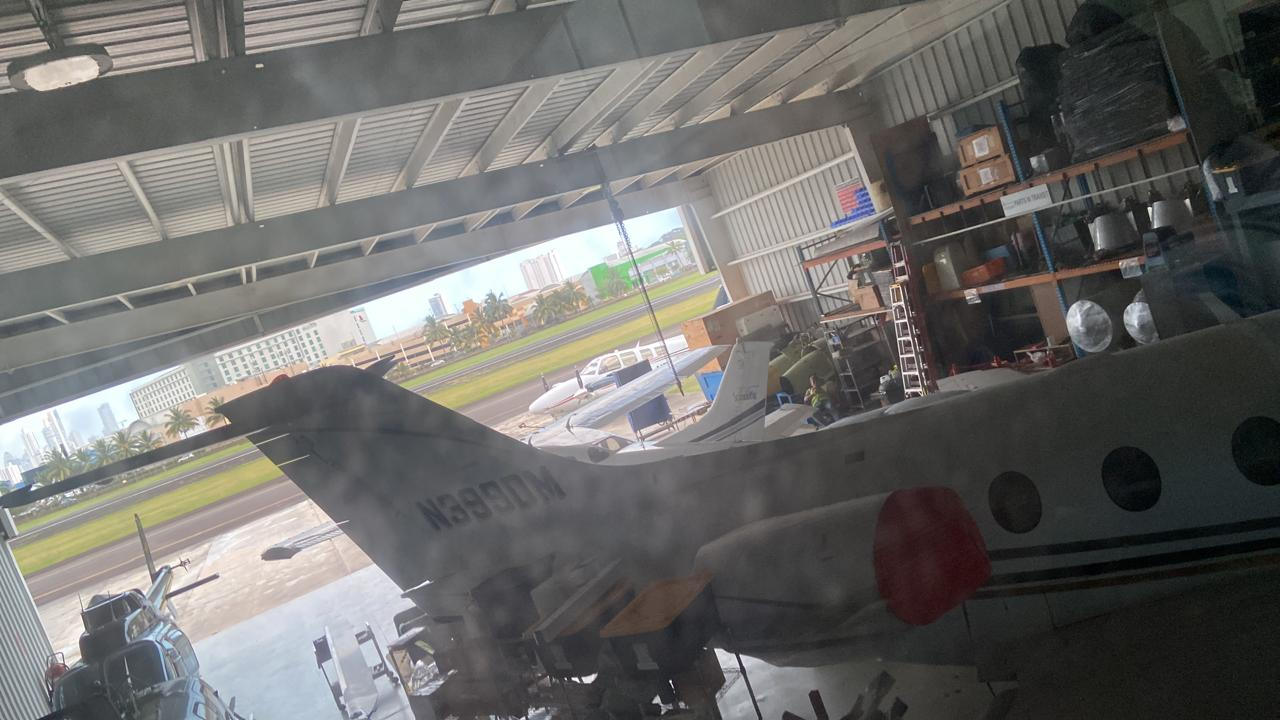
\includegraphics[width=0.6\textwidth]{prac/hang.jpg} % Change to your image filename
    \caption{Parte inferior del hangar.}
    \label{hangar}
\end{figure}
\newpage
\subsection{Ubicación.}
Air Logistics Corp. Se encuentra ubicada en el Aeropuerto Internacional de Albrook, Ciudad de Panamá, República de Panamá. 
\begin{figure}[h] % 'h' means "here", LaTeX tries to place it here
    \centering
    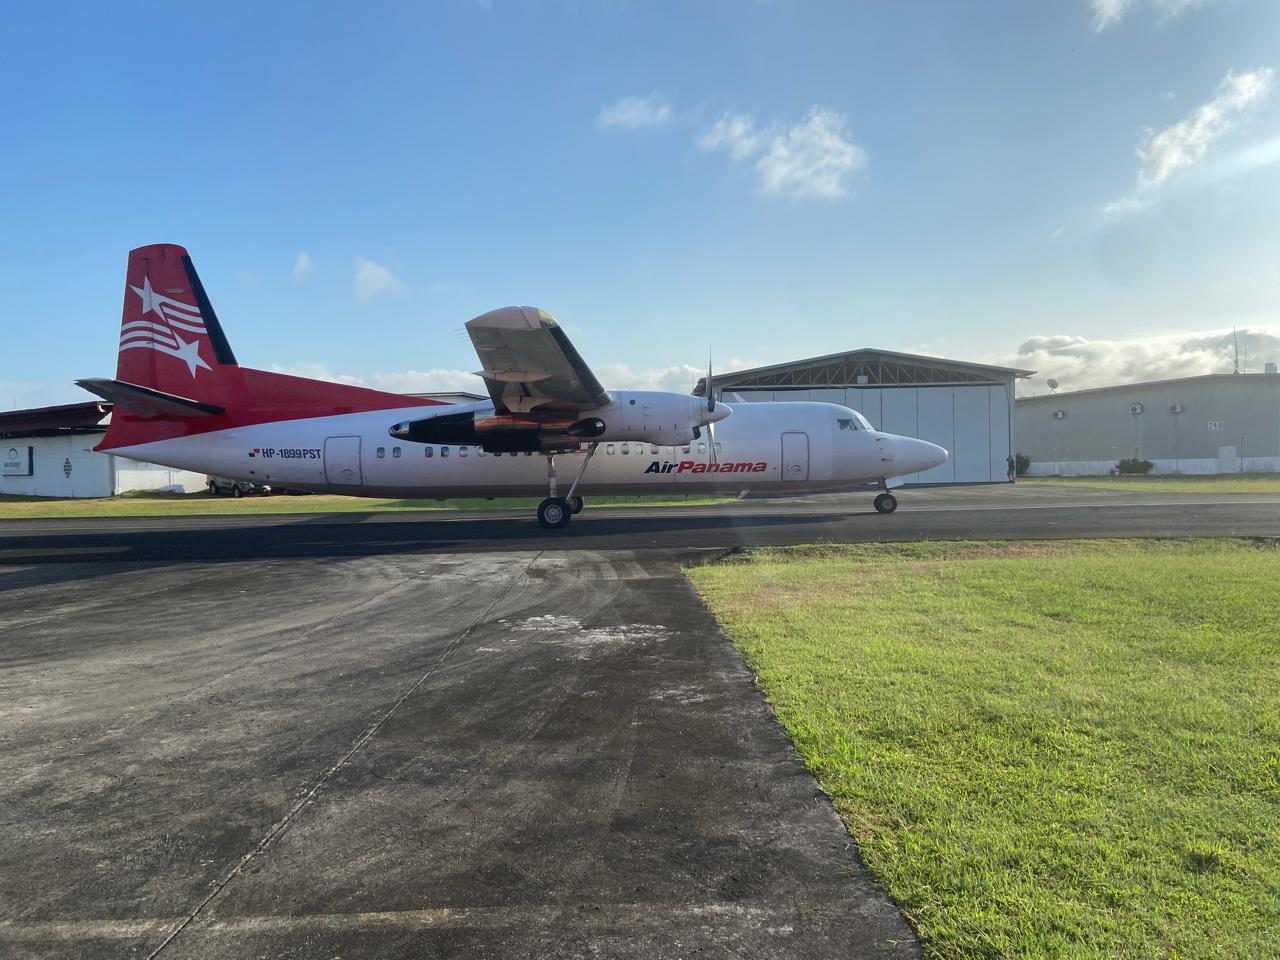
\includegraphics[width=0.6\textwidth]{prac/aerop.jpg} % Change to your image filename
    \caption{Pista secundaria del aeropuerto.}
    \label{logoAIRLOG}
\end{figure}